%!TEX root = ../thesis.tex
%*******************************************************************************
%****************************** Second Chapter *********************************
%*******************************************************************************

\chapter{Related Work}

\ifpdf
    \graphicspath{{04_Chapter2/Figs/Raster/}{04_Chapter2/Figs/PDF/}{04_Chapter2/Figs/}}
\else
    \graphicspath{{04_Chapter2/Figs/Vector/}{04_Chapter2/Figs/}}
\fi

This section covers current methods solving Bayesian Optimization in high dimensions that are considered state-of-the-art.
This is not an exhaustive review. 
For each algorithm, I discuss the effectiveness with regards to the dataset or function that the respective paper does the evaluation on.

Unless specified differently, I use the following terminology during my discussion.

\begin{enumerate}
\item $f$ is the real function to be optimized. Often I will use the term approximate, as many algorithms rely on a surrogate approximation of the function $f$ such that the global optimum can be found.
\item Assuming the function $f$ is of the form $f(x) = y$ with $x \in \mathbf{R}^D$, where $D$ denotes the dimensionality of $x$, then we define the optimized value of $f$ to be $x^* = \arg \max_{x} f(x)$.
\item $g$ and any subscripted or superscripted derivative of $g$ is a component that one uses to approximate $f$.
\item Anything that has a "hat" on (caret symbol on f is $\hat{f}$ ), refers to an empirical estimate. 
$\hat{f}$ would be an empirical estimate given datapoints $\mathit{D}$ of $f$.
\end{enumerate}

I will focus on three categories of Bayesian Optimization algorithms: Algorithms that make use of a projection matrix, algorithms that, algorithms that exploit additive substructures and "additional approaches" that are uncategorised.

\section{Projection matrix based algorithms}

In my work, I focus on algorithms that optimize the black box function $f$ by using a lower-dimensional projection.
I proceed with discussing some algorithms that I have implemented for my experiments in the next subsection (all except the algorithm "Active learning of linear subspaces").
I will briefly describe additional interesting algorithms that raise interesting ideas for possible future work afterwards.
For this family of algorithms, the approximation is a function of $f(x) \sim g(x; A)$, where the properties of $A$ are algorithm-specific.
The following descriptions aims at giving a brief overview at the methods at hand. 
I refer the curious reader to the individual paper for a more detailed and formal description of the respective topic.

\subsection{Active learning of linear subspaces}

\begin{algorithm}
\caption{Simultaneous active learning of functions and their linear embeddings (pseudocode) :: Active learning of linear subspace \citep{Garnett2013}}

\begin{algorithmic} 
\REQUIRE $d, D;$ kernel $\kappa$, mean function $\mu$; prior $p(R)$ 
\STATE $X \leftarrow \emptyset$
\STATE $Y \leftarrow \emptyset$

\WHILE{budget not depleted}
\STATE $ q(R) \leftarrow \text{LAPLACEAPPROX}( p(R | X, Y, \kappa, \mu) ) $
\STATE $ q(f) \leftarrow  APPROXMARGINAL( p(f | R), q(R)) $
\STATE $ x_* \leftarrow OPTIMIZEUTILITY( q(f), q(R) )$
\STATE $ y \leftarrow OBSERVE( f( x_* ) ) $
\STATE $ X \leftarrow [X; x_*] $
\STATE $ Y \leftarrow[Y; y_*] $
\ENDWHILE

\RETURN $q(R), q(f)$
\end{algorithmic}

\end{algorithm}

\citep{Garnett2013} The assumption of this algorithm is that $f$ depends only on $ x := uR^T $ with $ R \in \mathbf{R}^{d \times D}$, $ u \in \mathbf{R}^d $ and where $d << D$. 
The algorithm learns a projection matrix $R$ and the surrogate function$g(u)$, with $f(x) \sim g(u) $. \\

The \textbf{Laplace approximation} for $R$ is using the mode of the probability distribution $\log P (R | D) $ as a mean, and the covariance is taken as the inverse Hessian of the negative logarithm of the posterior evaluated at the mean of the distribution.
Together, this describes the probability distribution $p(R|X, Y, \kappa, \mu )$, where $\mu$ is the mean function, and $\kappa$ is the covariance function.\\

% TODO: be more accurate here
The \textbf{approximate marginal} subroutine is a novel method proposed in the paper that integrates over the different parameters in the paper.
This marginal approximation does a local expansion of $q(x_* | \theta) $ to $p(x_* | D, \theta)$. \\

The \textbf{sequential optimization of utility} (choice of next best point) is done using Bayesian Active Learning by disagreement, where the utility function is the expected reduction in the mutual information, as opposed to uncertainty sampling reducing entropy, which  is not well defined for all values. \\

The metrics used in this paper are negative log-likelihoods for the test points, and the mean symmetric kullback leiber divergence between approximate and true posteriors.
The proposed method always outperforms the naive MAP method for the presented functions close to a factor of 2 for both loss functions.
Tests are conducted on a real, and synthetic dataset with up to $D = 318$ and selecting $N = 100$ observations. 

\subsection{Random embeddings (REMBO)}
REMBO is an algorithm that allows the optimizer to search in a smaller search space.
The result of the optimized value $x^*$ is then projected to the higher dimensional space (including projections), to retrieve the actual optimized argmax value of the function $f$. 
More specifically, REMBO proposes the following model for Bayesian Optimization: \\

\citep{Wang2013} Let $x \in \mathbb{R}^D$ and $y \in \mathbb{R}^d$. Assume, that $f(x) = g(Ay)$. We can generate $A \in \mathbb{R}^{D \times d}$ by randomly generating this matrix.
$A$ must have the property that $A^T \times A = I$, where $I \in \mathbf{R}^{d \times d}$ denotes the identity matrix with $d$ diagonal elements.
The space over which the user searches, as such, is $d$-dimensional.
This implies that REMBO is more efficient in sampling datapoints, and learning the structure of a neighborhood in the high-dimensional space (by using the neighborhood of the low-dimensional space). \\

\begin{figure}[H]
    \centering
        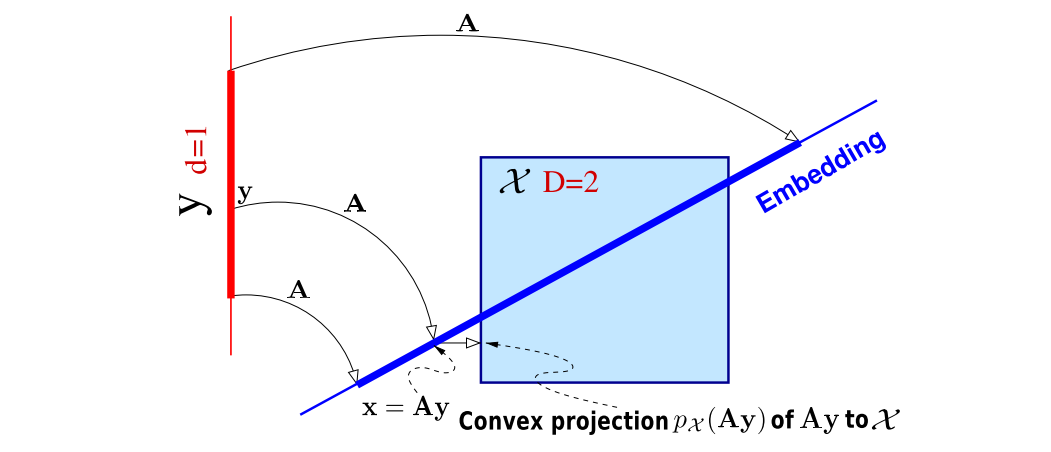
\includegraphics[width=\textwidth]{rembo_convex_projection.png}
        \caption{Parabola Original}
        \label{fig:gull}
    \caption{
    Source \citep{Wang2013}: Embedding from $d = 1$ into $D=2$.
    The box illustrates the 2D constrained space $\mathbf{X}$, while the thicker red line illustrates the 1D constrained space $\mathbf{Y}$.
    Note that if $A \times y$ is outside of $\mathbf{X}$, it is projected onto $\mathbf{X}$ using a convex projection.
    The set $\mathbf{Y}$ must be chosen large enough so that the projection of its image, $A \times y $ with $y \in \mathbf{Y}$, onto the effective subspace (vertical axis in this diagram) covers the vertical side of the box.
    }\label{fig:animals}
\end{figure}

The elegance of REMBO lies in the fact that the matrix $A$ can be chosen as a random orthogonal matrix.
The authors argue with an empirical proof, that if the optimization domain's parameters are well-chosen, that the chance of getting a bad projection matrix has a certain threshold. \\

I now proceed with a more formal treatment of the intuitive concept explained above: \\

\cite{Wang}
A function $f : \mathbf{R}^D \rightarrow \mathbf{R}$ is said to have effective dimensionality $d_e$ (where $d_e < D$), if there exists a linear subspace $\mathcal{T}$ of dimension $d_e$ such that for all $ x_\top \in \mathcal{T} \subset \mathbf{R}^D $ and $x_\perp \in \mathcal{T_\perp} \subset \mathbf{R}^D $, we have $ f(x) = f(x_\top +x_\perp ) = f(x_\top)$.
$\mathcal{T^\perp}$ is the orthogonal complement of $\mathcal{T}$.

Assume $ f : \mathbf{R}^D \rightarrow \mathbf{R} $ has effective dimensionality $d_e$.
Given a random matrix $ \mathbf{A} \in \mathbf{R}^{D \times d} $ (where $d \geq d_e$) with independent entries sampled from $ \mathcal{N}(0, 1) $.
For any $ x \in \mathbf{R}^D $, there exists a $y \in \mathbf{R}^d $ such that $ f(x) = f(\mathbf{A} y ) $.
The user now only need to optimize over all possible $y \in \mathbf{R}^d$, instead of all possible $x \in \mathbf{R}^D $. \\


\begin{figure}[H]
    \centering
        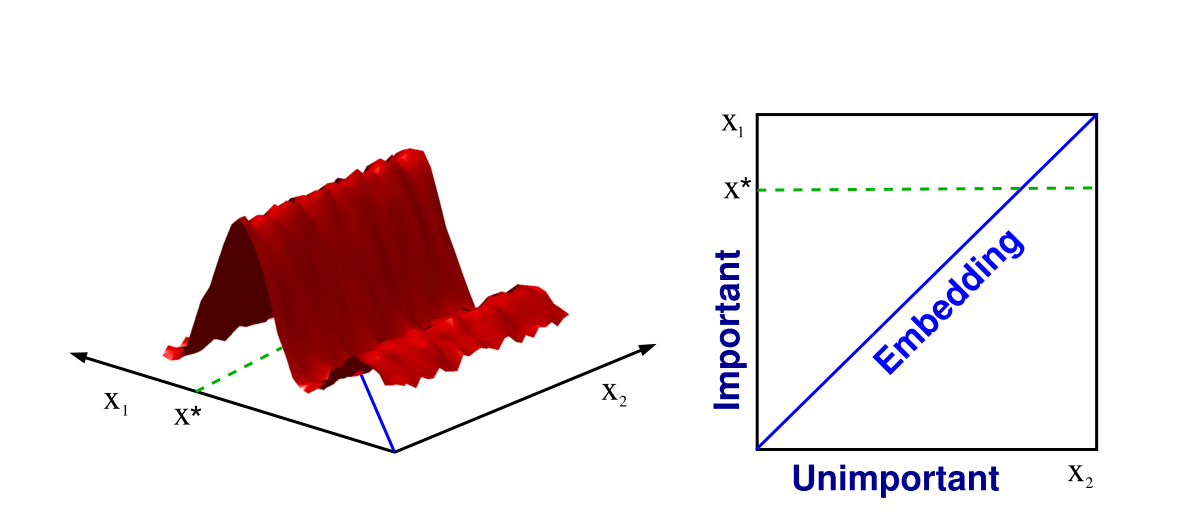
\includegraphics[width=\textwidth]{rembo_sinus_function.png}
        \caption{Parabola Original}
        \label{fig:gull}
    \caption{
    Source \citep{Wang2013}: This function in D=2 dimesions only has d=1 effective dimension.
    Hence, the 1-dimensional embedding includes the 2-dimensional function’s optimized value $x^*$. 
    It is more efficient to search for the optimum along the 1-dimensional random embedding than in the original 2-dimensional space.
    }\label{fig:animals}
\end{figure}

REMBO has a fairly high probability of failing (more than 20\% in the experiments conducted in the paper) by choosing an $A$ that lies orthogonal the the directions of highest change in the function $f$.
The authors propose interleaved runs, where for each $k$'th point selection, a differently sampled orthogonal random matrix is chosen. 
The probability of generating a bad embedding lower with higher $k$.
However, each $k$ has a set of observations $X$ which is not shared across the different interleaved runs. \\
Extensions to REMBO include \citep{RemboExtension}.

\subsection{Applications to high-dimensional uncertainty propagation}
I put most emphasis on this algorithm during my experiments. 
As such, I will be more detailed with the description of this algorithm. \\

\citep{Tripathy} This algorithm assumes that  $f(x) \sim g( \mathbf{W}^T y)$ where $ \mathbf{W} \in \mathbb{R}^{D \times d} $ and $D >> d$.
$ \mathbf{W} $ again has the property that $\mathbf{W^T}  \times \mathbf{W} = I$ where $I \in \mathbf{R}^{d \times d}$ denotes the identity matrix in $d$ dimensions. 
This algorithm does not require gradient-information.
This makes it easier to implement, and more robust to noise according to the authors of this paper. \\


I refer to the set of kernel parameters and the GP noise variance as GP-hyperparameters.
I refer to the projection matrix $ \mathbf{W} $ as the projection matrix.

The GP noise variance, kernel parameters and  $ \mathbf{W} $ can be found iteratively.
The main idea of the algorithm is to first fix both the kernel parameters and the GP noise variance, and identify $ \mathbf{W} $.
Then, we fix $ \mathbf{W} $ and train over the GP-hyperparameters.
This procedure is repeated until the change of the log-likelihood between iterations is below some $ \epsilon_l $, or if the maximum number of steps of optimization is reached.
We repeat this procedure many times (as dictated by the number of restarts).
Empirially, the probability of finding a good projection increases with the number of restarts, and the maximum number of iterations the algorithm is allowed to take during the optimization of the joint parameter set $\mathbf{W}$ and the hyperparameters (as given in the next paragraphs).\\

\paragraph{I now proceed with a more formal description of the algorithm.}
The quantities of interest are

\begin{align}
\mu_f &= \int f(x) p(x) dx \\
\sigma^2_f &= \int ( f(x) - \mu_f )^2 p(x) dx \\
f \sim p(f) &= \int \delta( f - f(x) ) p(x) dx
\end{align}

The authors assume that w.l.o.g., the search space of the projection matrices can be restricted to matrices on the siefel manifold.
The argument for this is that the projected subspace does not change, merely the representation of the subspace.
Here, the family of orthogonal matrices of dimension $d \times D$ is denoted by $\mathbf{W} \in V_d(\mathbb{R}^D) $.
This quantity is also known as the \textbf{Stiefel manifold} \citep{StiefelBayesianInference} \citep{StatisticsStiefelIntro} \citep{StiefelNonparametric}, where $d$ is the found effective dimension of the function, and $D$ is the real input dimension to the function. \\

\subsubsection{The Matern32 Kernel}
The optimization processes in the paper use the Matern-32 kernel function.
This function has two input vectors $a$ and $b$.

\begin{align}
K(a,  b, \theta) = s^2 \left( 1 + \sqrt{3} \sum_{i=1}^l \frac{(a_i - b_i)^2}{ \textit{l}_i} \right) exp\left( - \sqrt{3} \sum_{i=1}^l \frac{(a_i - b_i)^2}{ \textit{l}_i} \right)
\end{align}

Because I want to avoid numerical testing and implementation, I use the derivative as provided in the GPy library.
The $s, l_1, \ldots, l_l $ are hyper-parameters of the kernel, referred to as the kernel-variance, and the kernel-lengthscales. 
The concatenated vector of all these kernel hyperparameters is denoted by $\phi$. \\

The only modification made to this kernel is the additional parameter $W$:

\begin{equation}
k_{AS} : \mathbb{R}^D \times \mathbb{R}^D \times V_d(\mathbb{R}^D) \times \phi -> \mathbb{R} \\
\end{equation}
\text{where the kernel has the form}
\begin{equation}
k_{AS} (x, x'; W, \phi) = k_d(W^T x, W^T x'; \phi)
\end{equation}

\subsection{Overview of the algorithm}

In the following, I will explain the individual steps of the algorithm.
The shown two steps are repeated until the change of the log-likelihood reaches a certain threshold.
This algorithm is repeated a number of restarts, as the initial sample of $W$ plays a big role in finding a good converged embedding.

\subsubsection{Step 1.: Determine the active projection matrix W}
In this step, the algorithm optimizes $W \in V_d(\mathbb{R}^D)$ while keeping the kernel hyperparameters $\phi$ and the GP noise variance $s_n$ fixed.

To simplify calculations later, we define the function, where all parameters but $W$ are fixed as $F$. 
The other parameters are determined from previous runs, or are freshly sampled:

\begin{align}
F(W) &:= \mathcal{L}(W, \phi, s_n; X, y) \\
& = \log p(y | X, W, \phi, s_n) \\
& =  -\frac{1}{2} (y - m)^T (K + s_n^2 I_N)^{-1} (y - m) -\frac{1}{2} \log|K + s_n^2 I_N| -\frac{N}{2} \log 2 \pi   \\
\end{align}

where $\phi, s_n; X, y$ are fixed and $m$ is the prior mean function, which is 0 in our specific case.

To optimize over the loss function, the algorithm defines the derivative of $F$ with regards to each individual element of the weights-matrix:

\begin{align}
\nabla_{w_{i,j}} F(W) &:= \nabla_{w_{i,j}} \mathcal{L}(W, s_n; X, y) \\
& = \frac{1}{2} \text{tr} \left[ \{ (K + s_n^2 I_N)^{-1} (y-m) \left( (K + s_n^2 I_N)^{-1} (y-m) \right)^T - (K + s_n^2 I_N)^{-1} \} \nabla_{w_{i,j}} (K + s_n^2 I_N) \right]
\end{align}

both these functions depend on the kernel $K$, and it's derivative $\nabla_{w_{i,j}} K$. \\

To optimize over $F$, a more sophisticated algorithm is used, that resembles iterative hill-climbing algorithms.
First, the paper defines the function whose output is a matrix in the Stiefel manifold

\begin{equation}
\gamma(\tau; W) = (I_D - \frac{\tau}{2} A(W) )^{-1} (I_D + \frac{\tau}{2} A(W) ) W
\end{equation}


where $W$ is a fix parameter, and $\tau$ is the variable which modifies the direction that we move on in the Stiefel manifold and with

\begin{equation}
A(W) = \nabla_{W} F(W) W - W ( \nabla_{W} F(W) )^T
\end{equation}

One iteratively chooses fixed $W$, and does a grid-search over $\tau$ such that at each step, the log-likelihood $\mathcal{L}$ is increased.

\subsubsection{Step 2.: Optimizing over GP noise variance and the kernel hyperparameters}

We determine the hyperparameters by optimizing over the following loss function, where $X$ are the input values, $Y$ are the corresponding output samples. $\phi$ is the vector of the kernel hyperparameters and $s_n$, the GP noise variance. \\

One keeps the $W$ fixed (either by taking $W$ from the last iteration, or freshly sampling it), and then defines the loss function

\begin{equation}
	L(\phi) = \mathcal{L}(W, \phi, s_n; X, y) 
\end{equation}

To optimize this loss function, a simple optimization algorithm such as $L-BFGS$ is used to individually maximize each element of the hyperparameter vector with regards to the log-likelihood.
This is done for a maximum number of steps, or until the change of improvement becomes marginal. \\

\subsubsection{Additional details}
Because initialization is a major factor in this algorithm, these steps are iteratively applied for many hundred steps.
There are also many tens or hundreds of restarts to ensure that the search on the Stiefel manifold results in a good local optimum, and does not get stuck on a flat region with no improvement.
This algorithm is very sensitive on the initially sampled parameter $W$.

\subsubsection{Identification of active subspace dimension }
One cannot know the real active dimension of a problem that one does not know the solution to.
As such, the proposed to apply the above algorithms iteratively by increasing the selected active dimension $d$.
The moment where the relative change between the best found matrix between two iterations is below a relative threshold $\epsilon_s$, the previous active dimension is chosen as the real active dimension. 
The algorithm identifies the loss for each possible active dimension.
It then chooses a dimension, where the relative difference to the previous loss (of the one-lower dimension) is below a certain threshold.

\section{Algorithms that exploit additive substructures}

Functions with additive substructures can be decomposed into a summation over subfunctions, such that
$ f(x) \sim g_0(x) + g_1(x) + \ldots g_2(x) $ where each $g_i$ may operate only on a subset of dimensions of $x$.

\subsection{Independent additive structures within the target function}
% TODO: work on this algorithm a little more extensively, such that you can show the intuition, and potentially a short algorithm outline

\citep{Gardner2017} Assume that $f(x) = \sum_{i=1}^{ |P| } f_i (x[P_i] )$, i.e. $f$ is fully additive, and can be represented as a sum of smaller-dimensional functions $f_i$, each of which accepts a subset of the input-variables.
The kernel also results in an additive structure: $f(x) = \sum_{i=1}^{ |P| } k_i (x[P_i], x[P_i])$.
The posterior is calculated using the Metropolis Hastings algorithm.
The two actions for the sampling algorithm are 'Merge two subsets', and 'Split one set into two subsets'.
$k$ models are sampled, and we respectively approximate $p(f_* | D, x^*) = \frac{1}{k} \sum_{j=1}^{k} p( f(x^* | D, x, M_j) )$, where $M_j$ denotes the partition amongst all input-variables of the original function $f$.

\section{Additional approaches}

\subsection{Elastic Gaussian Processes}
% TODO: Shortly touch on this, give an intuition, but nothing more

\citep{Rana2017} Use a process where the space is iteratively explored.
The key insight here is that with low length-scales, the acquisition function is extremely flat, but with higher length-scales, the acquisition function starts to have significant gradients.
The two key-steps is to 1.) additively increase the length-scale for the gaussian process if the length-scale is not maximal and if $|| x_{init} - x^* || = 0$.
And 2.) exponentially decrease the length-scale for the gaussian process if the length-scale is below the optimum length-scale and if $|| x_{init} - x^* || = 0$.

\subsection{High dimensional Gaussian bandits}

\citep{Djolonga2013} This model assumes that there exists a function $g : \mathbf{R}^k \implies [0, 1]$ and a matrix $A \in \mathbf{R}^{d \times D}$ with orthogonal rows, such that $f(x) \sim g(Ax) $. Assume $g \in \mathcal{C}^2$. 
% Assume that $B = \mathbf{B}^D (1 + \epsilon ) $.
% We want to maximize $f: B \implies [0, 1] $.\\

The algorithm identifies $A$ by the 

\begin{algorithm}
\caption{The SI-BO algorithm \citep{Djolonga2013}}

\begin{algorithmic} 
\REQUIRE $m_X, m_{\Phi}, \lambda, \epsilon, k$, oracle for the function $f$, kernel $\kappa$ 

\STATE $C \leftarrow m_X $ samples uniformly from $\mathbb{S}^{d-1}$

\FOR{$ i \leftarrow 1$ to $m_X$}
\STATE $\Phi_i \leftarrow m_{\Phi}$ samples uniformly from $\{ -\frac{1}{\sqrt{m}}, \frac{1}{\sqrt{m}} \}^k$
\ENDFOR

\STATE $ y \leftarrow $ (compute using Equation 1 -- INSERT Eq 1 here, or create a summary of all important equations here)

\STATE select $z_i$ according to a UCB acquisition function, evaluate $f$ on it, and add it to the datasamples found so far

\end{algorithmic}

\end{algorithm}

The SI-BO algorithm consists of a subspace identification step, and an optimization step using GP-UCB.

% TODO: understand this part of the paper better

The \textbf{subspace identification} is treated as a low-rank matrix recovery problem as presentedin \citep{CevherSubspaceIdentificationKrause}.



\subsection{Bayesian Optimization using Dropout}
% TODO: Shortly touch on this, give an intuition, but nothing more

\citep{Li2018} propose that the assumption of an active subspace is restrictive and often not fulfilled in real-world applications.
They propose three algorithms, to iteratively optimize amongst certain dimensions that are not within the $d$ 'most influential' dimensions: 1.) Dropout Random, which picks dimensions to be optimized at random, 2.) Dropout copy, which continuous optimizing the function values from the found local optimum configuration, and 3.) which does method 1. with probability $p$, and else method 2.
The $d$ 'most influential' dimensions are picked at random at each iteration. \\

Additional works I explored as background research or additional methods include \citep{KernelGibbsSampler}, \citep{VirtualVsReal}, \citep{SensorPlacement}, \citep{BatchedBO}, \citep{GPforML}.
